{% -*- mode: LaTeX; TeX-PDF-mode: t; TeX-master: "manual"; -*-
}

\chapter{\ei Clients}
\label{ch:clients}

This chapter describes the different clients available by default in
the \ei framework. Currently the only mature one is the web-client
that we describe in Section~\ref{ch:clients:web}. The Eclipse and
remote shell clients are still under development.

\begin{figure}[h]
\hrule\smallskip
\begin{center}
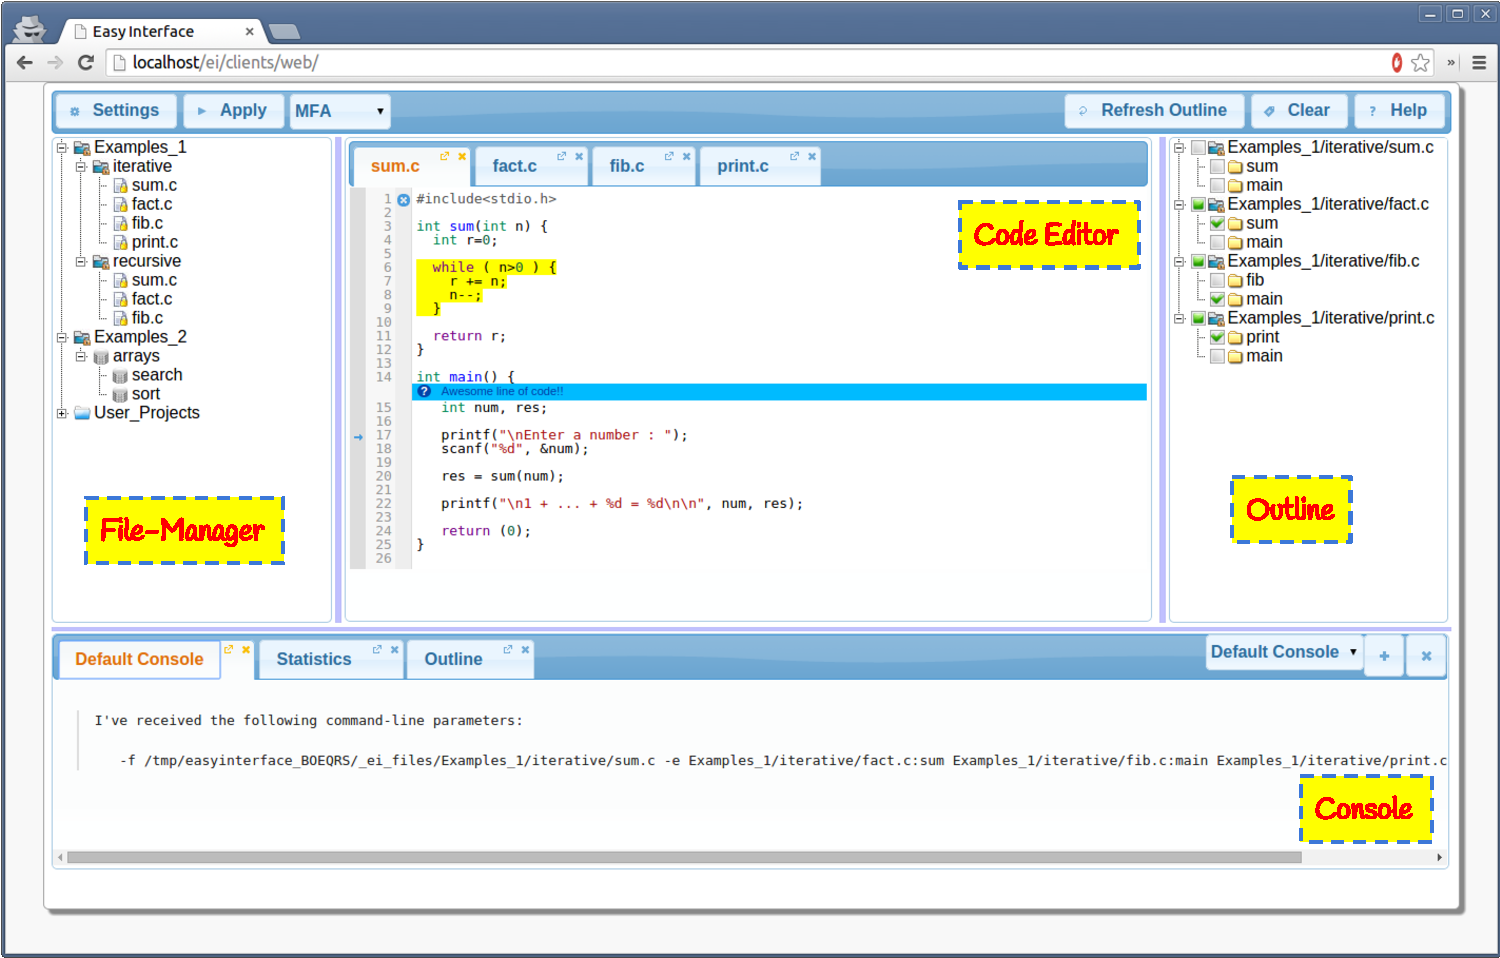
\includegraphics[width=1\textwidth]{fig/webclient.pdf}
\end{center}
\caption{\ei Web Client}
\label{fig:webclient}
\hrule
\end{figure}

\section{The Web-Client}
\label{ch:clients:web}

The web-client of \ei is a Java script based developing environment
that runs in a web browser. To access it simply visit
\url{http://localhost/ei/clients/web}, you will get a page similar to
that of Figure~\ref{fig:webclient}.

\subsection{Configuring the Web-Client}

The web-client has a configuration file to control, among others
things, which applications to include in the applications menu, which
examples to show in the file-manager, and how to generate the outline
for a given program.
%
By default the web-client looks for the configuration file
\texttt{clients/web/webclient.cfg}, and if it does not exists it uses
\texttt{clients/web/webclient.default.cfg}.
%
It is recommended not to substantially change
\texttt{webclient.default.cfg}, instead create your own
\texttt{webclient.cfg}. 

In what follows, when we refer the \emph{default server} we mean the
one that is available at the same address as web-client, i.e., if the
web-client was accessed using the URL
``\lst{http://somedomain/.../ei/client/web}'' then the URL of the
default server is ``\lst{http://somedomain/.../ei/server}''.

The configuration file is a text file that includes a single JSON
record of the following form:

\bigskip
\begin{lstlisting}
{
  (*title*): (*"Easy Interface"*),
  (*apps*): (*[\{server: "http://domain/.../ei/server, apps: ["myapp", "costa", "mhp"]\}, ... ]*),
  (*examples*): (*[\{server: "http://domain/.../ei/server, examples: ["mhpex","costex"]\}, ... ]*),
  (*outlineserver*): (*"http://domain/.../ei/server"*),
  (*outlineapp*): (*"coutline"*)
}
\end{lstlisting}

\bigskip
\noindent
All fields in the above record are optional, the web-client assigns
default values for those that are not available. Let us explain the
meaning of the above fields:

\begin{itemize}

\item \texttt{title}: is used to set the window title (see
  Figure~\texttt{fig:webclient}). The default value is ``Easy
  Interface'';

\item \texttt{apps}: is used to change the set of application to be
  listed in the applications menu. Its value is a list of JSON records
  of the form
%
  \begin{center}
    \texttt{\{server: SRV, apps: APPSLIST\}} 
  \end{center}
  % 
  where \lst{SVR} is a URL to an \ei server and \lst{APPSLIST} is a
  list of application identifiers (see
  \xmlstructref{server}{APP}). \lst{APPSLIST} can also be the special
  value \lst{_all} which refer to all application of the corresponding
  server. The default value of this field is a list with a record that
  refers to all application of the default server.

\item \texttt{example}: is used to change the set of examples to be
  listed in the file-manager area. Its value is a list of JSON records
  of the form
%
  \begin{center}
    \texttt{\{server: SRV, examples: EXLIST\}} 
  \end{center}
  % 
  where \lst{SVR} is a URL to an \ei server and \lst{EXLIST} is a list
  of example set identifiers (see
  \xmlstructref{server}{exset}). \lst{EXLIST} can also be the special
  value \lst{_all} which refer to all example sets of the
  corresponding server. The default value of this field is a list with
  a record that refers to all example sets of the default server.

\item \texttt{outlineserver} and \texttt{outlineapp}: are used to
  indicate which application to use for generating the outline (see
  Section~\ref{ch:clients:web:outline}). The default value of
  \texttt{outlineserver} is the default server, and the one of
  \texttt{outlineapp} is \texttt{coutline}.

\end{itemize}

\subsection{Generate Outline}
\label{ch:clients:web:outline}

The Outline App returns an XML with the outline tree.

%% 
\bigskip
\xmlstruct
{webclient}
{outline}
{
%
  Defines a list of points to be analysed.
\begin{itemize}
  \item \xmlstructattr{text} is the name to be show.
   \item \xmlstructattr{value} is the internalname .
\item \xmlstructattr{selectable} indicates if this node can be
  selected.
\item \xmlstructattr{icon} indicates an alternative path for the icon
  of the node.

\end{itemize}
%
}





\section{Eclipse Plugin}
\label{ch:clients:eclipse}

Under development. 

\section{Remore shell}
\label{ch:clients:shell}

Under development. 
